\documentclass[12pt,a4paper,titlepage]{article}
\usepackage[utf8]{inputenc}
\usepackage{polski}
\usepackage{listings}
\usepackage{graphicx}
\usepackage{xcolor}
\usepackage{minted}
\usepackage{amsmath}
\usepackage{caption}
 
\setminted{
    linenos=true,
    autogobble,
    breaklines,
    frame=lines,
    framerule=1pt,
    framesep=10pt
}

\newenvironment{longlisting}{}{}
 
\DeclareCaptionType{myequation}[][Równanie parametryczne]
\captionsetup[myequation]{labelformat=empty}

\makeatletter
\newcommand{\linia}{\rule{\linewidth}{0.4mm}}
\renewcommand{\maketitle}{\begin{titlepage}
    \vspace*{1cm}
    \begin{center}\small
    Politechnika Wrocławska\\
    Wydział Elektroniki\\
    Grafika Komputerowa i Komunikacja Człowiek-Komputer
    \end{center}
    \vspace{3cm}
    \noindent\linia
    \begin{center}
      \LARGE \textsc{\@title}
         \end{center}
     \linia
    \vspace{0.5cm}
    \begin{flushright}
    \begin{minipage}{7cm}
    \textit{\small Autor:}\\
    \normalsize \textsc{\@author} \par
    \end{minipage}
    \vspace{5cm}

     {\small czwartek, 17\textsuperscript{15}-20\textsuperscript{15} TN}\\
        mgr inż. Szymon Datko
     \end{flushright}
    \vspace*{\stretch{6}}
    \begin{center}
    \@date
    \end{center}
  \end{titlepage}%
}
\makeatother
\author{Justyna Skalska, 225942}
\title{Sprawozdanie nr 4\\
(OpenGL - oświetlanie scen 3D)}

\begin{document}

\maketitle
\section{Omówienie tematu}
Naszym zadaniem na laboratoriach było stworzenie prostego programu wprowadzającego do oświetlania obiektów w scenach 3D z wykorzystaniem OpenGL wraz z rozszerzeniem GLUT. Głównym zadaniem było oświetlenie modelu jajka przy wykorzystaniu modelu Phonga zadanego wzorami podanymi w instrukcji. Program miał oświetlać obiekt dwoma źródłami światła o innych kolorach. Obiekt powinien się także obracać przy użyciu myszy. Ostatnim zadaniem było przemieszczanie źródeł światła dookoła jajka za pomocą obu przycisków myszy.

\begin{myequation}[H]
\begin{equation}
    \begin{split}
    & x_{u} = (-450u^4 + 900u^3 - 810u^2 + 360u - 45)cos(\pi v) \\
    & x_{v} = \pi(90u^5 - 225u^4 + 270u^3 - 180u^2 + 45)sin(\pi v) \\
    & y_{u} = 640u^3 - 960u^2 + 320u \\
    & y_{v} = 0 \\
    & z_{u} = (-450u^4 + 900u^3 - 810u^2 + 360u - 45)sin(\pi v) \\
    & z_{v} = -\pi(90u^5 - 225u^4 + 270u^3 - 180u^2 + 45)cos(\pi)
    \end{split}
\end{equation}
\caption{Równanie parametryczne wektorów normalnych modelu Phonga}
\end{myequation}

\section{Omówienie kodu}

\begin{listing}[H]
\caption{Zmienne globalne programu}
\begin{minted}[linenos,breaklines]{C++}
struct Point {   // punkt wykorzystywany przez program
  float x, y, z;
};
static GLfloat viewer[] = { 0.0, 0.0, 10.0 }; // położenie obserwatora
static int N = 30;  // liczba przedziałów
static Point** normals;  // tablica wektorów normalnych modelu Phonga
static GLint status = 0;    // stan klawiszy myszy 
\end{minted}
\end{listing}

\begin{listing}[H]
\caption{Funkcja wyliczająca wektory modelu Phonga}
\begin{minted}[linenos,breaklines]{C++}
Point getPhongVectors(float u, float v) {
    float x, y, z, x_u, x_v, y_u, y_v, z_u, z_v;

    x_u = (-450 * pow(u, 4) + 900 * pow(u, 3) - 810 * pow(u, 2) + 360 * u - 45) * cos(M_PI * v);
    x_v = M_PI * (90 * pow(u, 5) - 225 * pow(u, 4) + 270 * pow(u, 3) - 180 * pow(u, 2) + 45 * u) * sin(M_PI * v);
    y_u = 640 * pow(u, 3) - 960 * pow(u, 2) + 320 * u;
    y_v = 0;
    z_u = (-450 * pow(u, 4) + 900 * pow(u, 3) - 810 * pow(u, 2) + 360 * u - 45) * sin(M_PI * v);
    z_v = (- M_PI) * (90 * pow(u, 5) - 225 * pow(u, 4) + 270 * pow(u, 3) - 180 * pow(u, 2) + 45 * u) * cos(M_PI * v);

    x = y_u * z_v - z_u * y_v;
    y = z_u * x_v - x_u * z_v;
    z = x_u * y_v - y_u * x_v;

    float length = sqrt(pow(x, 2) + pow(y, 2) + pow(z, 2));

    x = x / length;
    y = y / length;
    z = z / length;

    return { x, y, z };
}
\end{minted}
\end{listing}

\begin{listing}[H]
\caption{Funkcja zwracająca dwuwymiarową tablicę wektorów normalnych modelu Phonga}
\begin{minted}[linenos,breaklines]{C++}
Point** getNormals(int n) {
    float interval = 1.0f / n;
    Point** vectorValues = new Point*[n + 1];

    for (size_t i = 0; i < n + 1; i++) {
        vectorValues[i] = new Point[n + 1];
    }

    for (size_t i = 0; i <= n; i++) {
        for (size_t j = 0; j <= n; j++) {
            float u = ((float)i) / n;
            float v = ((float)j) / n;

            vectorValues[i][j] = getPhongVectors(u, v);

            // przemnożenie każdej składowej wektora normalnego przez -1, aby go odwrócić, ponieważ wektory generowane przez funkcję są zawse zwrócone w jedną stronę
            if (i < n / 2) {
                vectorValues[i][j].x = (-1) * vectorValues[i][j].x;
                vectorValues[i][j].y = (-1) * vectorValues[i][j].y;
                vectorValues[i][j].z = (-1) * vectorValues[i][j].z;
            }
        }
    }

    return vectorValues;
}
\end{minted}
\end{listing}

\begin{listing}[H]
\caption{Funkcja rysująca jajko z trójkątów wraz z wektorami normalnymi modelu Phonga}
\begin{minted}[linenos,breaklines]{C++}
void drawEggFromTriangles(int n, Point** bezierValues, Point** normals) {
  glBegin(GL_TRIANGLES);

  for (size_t i = 0; i < n; i++) {
    for (size_t j = 0; j < n; j++) {
      glNormal3f(normals[i][j].x, normals[i][j].y, normals[i][j].z);
      glVertex3f(bezierValues[i][j].x, bezierValues[i][j].y - 5, bezierValues[i][j].z);
      glNormal3f(normals[i + 1][j].x, normals[i + 1][j].y, normals[i + 1][j].z);
      glVertex3f(bezierValues[i + 1][j].x, bezierValues[i + 1][j].y - 5, bezierValues[i + 1][j].z);
      glNormal3f(normals[i + 1][j + 1].x, normals[i + 1][j + 1].y, normals[i + 1][j + 1].z);
      glVertex3f(bezierValues[i + 1][j + 1].x, bezierValues[i + 1][j + 1].y - 5, bezierValues[i + 1][j + 1].z);
      
      glNormal3f(normals[i][j + 1].x, normals[i][j + 1].y, normals[i][j + 1].z);
      glVertex3f(bezierValues[i][j + 1].x, bezierValues[i][j + 1].y - 5, bezierValues[i][j + 1].z);
      glNormal3f(normals[i][j].x, normals[i][j].y, normals[i][j].z);
      glVertex3f(bezierValues[i][j].x, bezierValues[i][j].y - 5, bezierValues[i][j].z);
      glNormal3f(normals[i + 1][j + 1].x, normals[i + 1][j + 1].y, normals[i + 1][j + 1].z);
      glVertex3f(bezierValues[i + 1][j + 1].x, bezierValues[i + 1][j + 1].y - 5, bezierValues[i + 1][j + 1].z);
    }
  }

  glEnd();
}
\end{minted}
\end{listing}
\hfill \break
\hfill \break

\begin{longlisting}
\begin{minted}[linenos,breaklines]{C++}
void MyInit(void) {   
    // kod skopiowany z instrukcji laboratorium
    // - ustawienie parametrów materiału
    // - podstawowe składowe źródła światła
    // ...
  
    // kolor źródła
    const GLfloat COLOR_RED[] = { 1.0, 0.0, 0.0, 1.0 };
    const GLfloat COLOR_BLUE[] = { 0.0, 0.0, 1.0, 1.0 };
  
    // położenie źródła
    GLfloat light_position1[] = { 5.0, 10.0, 0.0, 1.0 };
    GLfloat light_position2[] = { 0.0, -10.0, 0.0, 1.0 };
    
    // pierwsze źródło światła
    glLightfv(GL_LIGHT0, GL_AMBIENT, light_ambient);
    glLightfv(GL_LIGHT0, GL_DIFFUSE, COLOR_RED);
    glLightfv(GL_LIGHT0, GL_SPECULAR, light_specular);
    glLightfv(GL_LIGHT0, GL_POSITION, light_position1);
    
    glLightf(GL_LIGHT0, GL_CONSTANT_ATTENUATION, att_constant);
    glLightf(GL_LIGHT0, GL_LINEAR_ATTENUATION, att_linear);
    glLightf(GL_LIGHT0, GL_QUADRATIC_ATTENUATION, att_quadratic);
    
    // kolejne źródło światła
    glLightfv(GL_LIGHT1, GL_AMBIENT, light_ambient);
    glLightfv(GL_LIGHT1, GL_DIFFUSE, COLOR_BLUE);
    glLightfv(GL_LIGHT1, GL_SPECULAR, light_specular);
    glLightfv(GL_LIGHT1, GL_POSITION, light_position2);
    
    glLightf(GL_LIGHT1, GL_CONSTANT_ATTENUATION, att_constant);
    glLightf(GL_LIGHT1, GL_LINEAR_ATTENUATION, att_linear);
    glLightf(GL_LIGHT1, GL_QUADRATIC_ATTENUATION, att_quadratic);

    // ustawienie opcji systemu oświetlania sceny 
    glShadeModel(GL_SMOOTH); // włączenie łagodnego cieniowania
    glEnable(GL_LIGHTING);   // włączenie systemu oświetlenia sceny 
    glEnable(GL_LIGHT0);     // włączenie źródła o numerze 0
    glEnable(GL_LIGHT1);     // włączenie źródła o numerze 1
    glEnable(GL_DEPTH_TEST); // włączenie mechanizmu z-bufora 
}
\end{minted}
\end{longlisting}
\begin{listing}
\caption{Funkcja inicjalizująca oświetlenie}
\end{listing}

\begin{listing}[H]
\caption{Funkcja renderująca scenę}
\begin{minted}[linenos,breaklines]{C++}
void RenderScene(void) {
    // czyszczenie okna aktualnym kolorem czyszczącym
    glClear(GL_COLOR_BUFFER_BIT | GL_DEPTH_BUFFER_BIT);
    
    // czyszczenie macierzy bieżącej
    glLoadIdentity();
    
    // zdefiniowanie położenia obserwatora
    gluLookAt(viewer[0], viewer[1], viewer[2], 0.0, 0.0, 0.0, 0.0, 1.0, 0.0);
    
    // narysowanie osi przy pomocy funkcji zdefiniowanej 
    Axes();
    
    glColor3f(1.0f, 1.0f, 1.0f);
    
    // jeśli lewy klawisz myszy wciśnięty
    if (status == 1) {
        // modyfikacja kąta obrotu o kat proporcjonalny do różnicy położeń kursora myszy
        theta += delta_x * pix2angle;
    }

    // obrót obiektu o nowy kąt
    glRotatef(theta, 0.0, 1.0, 0.0);
    
    drawEgg(N);
    
    MyInit();
    
    // przekazanie poleceń rysujących do wykonania
    glFlush();
    
    glutSwapBuffers();
}
\end{minted}
\end{listing}

\newpage
\section{Rezultat prac}
Udało mi się wykonać większość podpunktów zadania. Jajko zostało oświetlone dwoma źródłami światła, jednym - czerwonym, drugim - niebieskim. Obiekt obracał się wokół własnej osi po nieciśnięciu lewego przycisku myszy. Niestety z jakiegoś powodu jajko jest bardzo matowe. Nie udało mi się znaleźć rozwiązania tego problemu. Pokazane na rysunku \ref{fig:eggWithVectors} wektory normalne wydają się być wyliczone w odpowiedni sposób.

\begin{figure}[H]
\centering
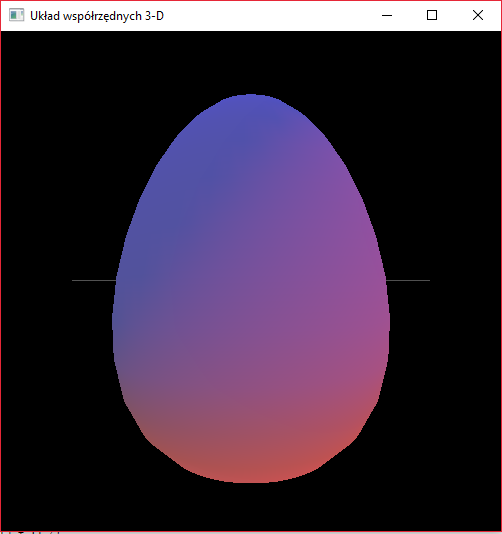
\includegraphics[width = 9cm]{images/egg_light.png}
\caption{Jajko oświetlone dwoma źródłami światła}
\label{fig:eggWithLight}
\end{figure}

\begin{figure}[H]
\centering
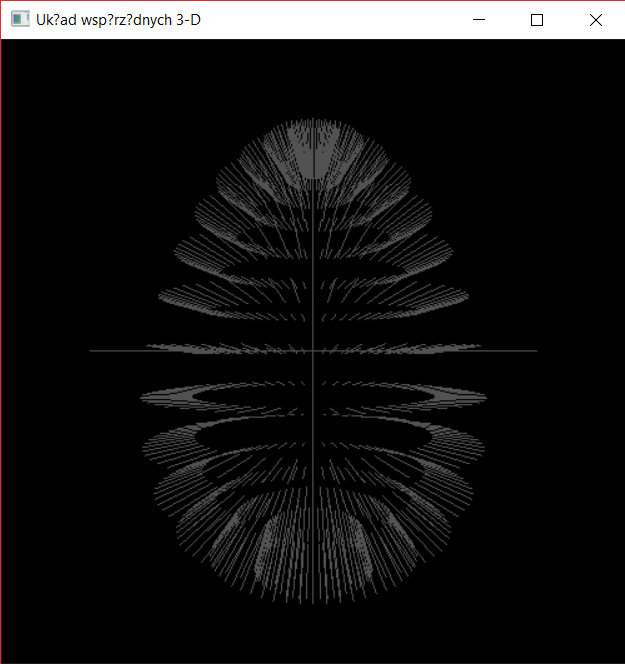
\includegraphics[width = 9cm]{images/egg_vectors.png}
\caption{Wizualizacja wektorów normalnych}
\label{fig:eggWithVectors}
\end{figure}

\end{document}
